\documentclass[a4paper, 12pt]{article}
\usepackage[a4paper,top=1.5cm, bottom=1.5cm, left=1cm, right=1cm]{geometry}
\usepackage{cmap}
\usepackage{mathtext}
\usepackage[T2A]{fontenc}
\usepackage[utf8]{inputenc}
\usepackage[english,russian]{babel}
\usepackage{multirow}
\usepackage{graphicx}
\usepackage{wrapfig}
\usepackage{tabularx}
\usepackage{float}
\usepackage{longtable}
\usepackage{hyperref}
\hypersetup{colorlinks=true,urlcolor=blue}
\usepackage[rgb]{xcolor}
\usepackage{amsmath,amsfonts,amssymb,amsthm,mathtools}
\usepackage{icomma}
\usepackage{euscript}
\usepackage{mathrsfs}
\usepackage{enumerate}
\usepackage{caption}
\usepackage{enumerate}
\mathtoolsset{showonlyrefs=true}
\usepackage{graphicx}
\usepackage{caption}
\usepackage{subcaption}
\usepackage{amsthm}
\usepackage[europeanresistors, americaninductors]{circuitikz}
\DeclareMathOperator{\sgn}{\mathop{sgn}}
\newcommand*{\hm}[1]{#1\nobreak\discretionary{}
	{\hbox{$\mathsurround=0pt #1$}}{}}

\newcommand{\framedtext}[1]{%
\par%
\noindent\fbox{%
    \parbox{\dimexpr\linewidth-2\fboxsep-2\fboxrule}{#1}%
}%
}

\title{\textbf{Определение удельного заряда электрона (3.3.1)}}
\author{Манро Эйден}
\date{}

\begin{document}

\maketitle

\newpage
\section*{А. Метод магнитной фокусировки}
\subsection*{Цель работы:}
Определение значения магнитных полей, при которых происходит фокусировка электронного пучка, и по результатам измерений считать удельный заряд электрона $e/m$.
\subsection*{В работе используются:}
Электронно-лучевая трубка и блок питания к ней; источник постоянного тока; соленоид; электростатический вольтметр; милливеберметр; ключи.

\subsection*{Теоретическая справка}
Здесь удельный заряд электрона определяется по формуле
\begin{equation}
\dfrac{e}{m_e} = \dfrac{8\pi^2V}{l^2} \left(\dfrac{n^2}{B_{\text{ф}}^2} \right),
\end{equation}
где $V$ - ускоряющий потенциал в электронной трубке, $l$ - путь электрона, $B_{\text{ф}}$ - фокусирующее поле, $n$ - номер фокуса.
\subsection*{Описание установки}
\begin{wrapfigure}{l}{0.2\textwidth}
  \begin{center}
    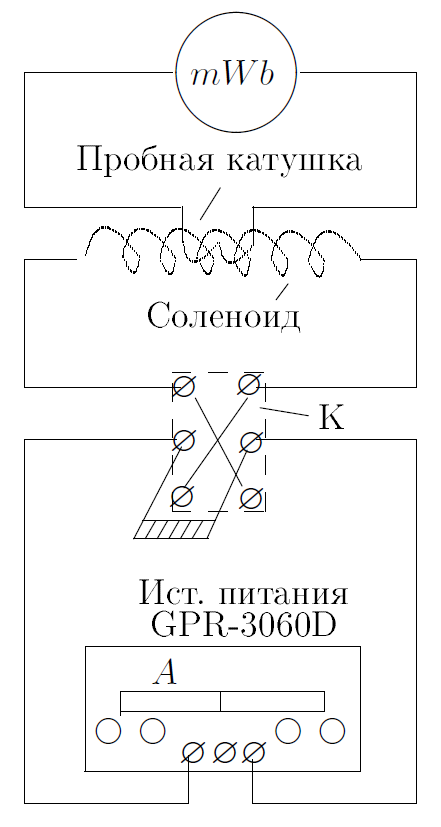
\includegraphics[width = 0.2\textwidth]{pictures/usta.png}
  \end{center}
  \textbf{\caption{Схема установки.}}
\end{wrapfigure}

Основной частью установки является электронный осциллограф, трубка которого вынута и установлена в длинном соленоиде, создающим магнитное поле. Напряжение на отклоняющие пластины и питание подводятся к трубке многожильным кабелем.

Пучок электронов, вылетающих из катода с разными скоростями, ускоряется анодным напряжением. Пропустив пучок сквозь две узкие диафрагмы, можно выделить электроны с практически одинаковой продольной скоростью. Небольшое переменное напряжение, поступающее с клеммы "Контрольный сигнал" осциллографа на отклоняющие пластины, изменяет только поперечную составляющую скорости. При увеличении магнитного поля линия на экране стягивается в точку, а затем снова удлиняется.

Магнитное поле создается постоянным током, величина которого регулируется ручками источника питания и измеряется амперметром. Ключ служит для изменения направления поля в соленоиде.

Величина магнитного поля определяется с помощью милливеберметра.

На точность результатов может влиять внешнее магнитное поле, особенно продольное.

Измерения магнитного поля с помощью милливеберметра обычно проводятся в предварительных опыта: при отключении ключа устанавливается связь между силой тока и индукцией магнитного поля в соленоиде.

\newpage
\;
\subsection*{Ход работы}

Для начала стоит определить связь между индукцией $B$ магнитного поля в соленоиде и током $I$ через обмотки магнита.

\begin{center}
    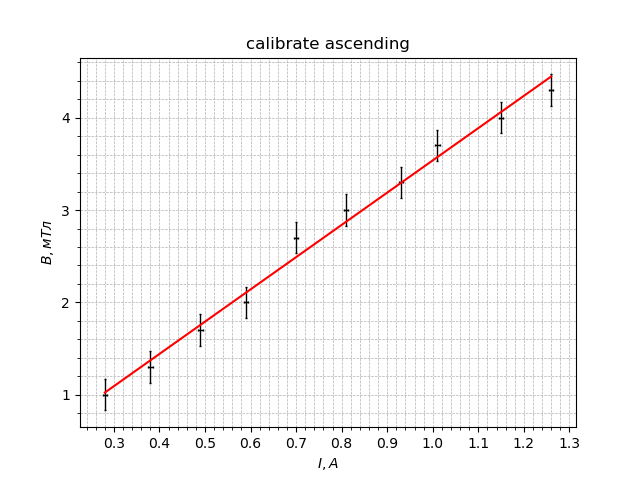
\includegraphics[width = 0.6\textwidth]{data/focus/graphs/ascend_calibrate.png}\\
    \textbf{График 1.} $B (I)$ в прямом направлении.
\end{center}

\begin{center}
    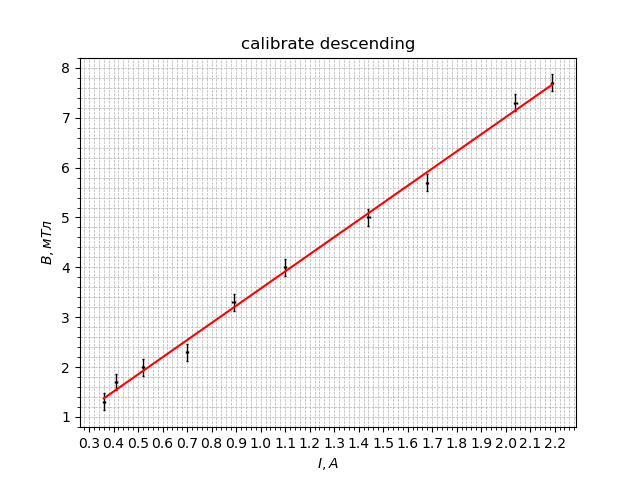
\includegraphics[width = 0.6\textwidth]{data/focus/graphs/descend_calibrate.png}\\
    \textbf{График 2.} $B (I)$ в обратном направлении.
\end{center}

\begin{equation}
    k_{B/I} = (3.60 \pm 0.07) \; \frac{\text{мТл}}{\text{А}} \; (\varepsilon = 2 \%)
\end{equation}

Теперь будем увеличивать постепенно ток и найдем ток при каждом фокусе, так как мы знаем зависимость $B = B(I)$ для каждого направления, то мы можем определить зависимость $B = f(n)$.

\begin{center}
    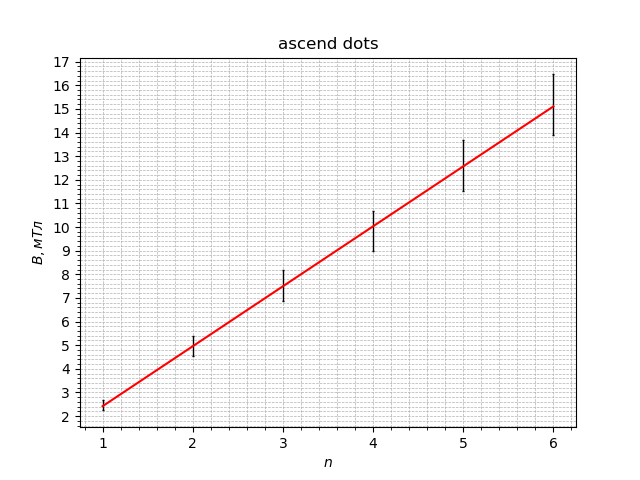
\includegraphics[width = 0.6\textwidth]{data/focus/graphs/ascend_dots.png}\\
    \textbf{График 3.} $B(n)$ в прямом направлении.
\end{center}

\begin{center}
    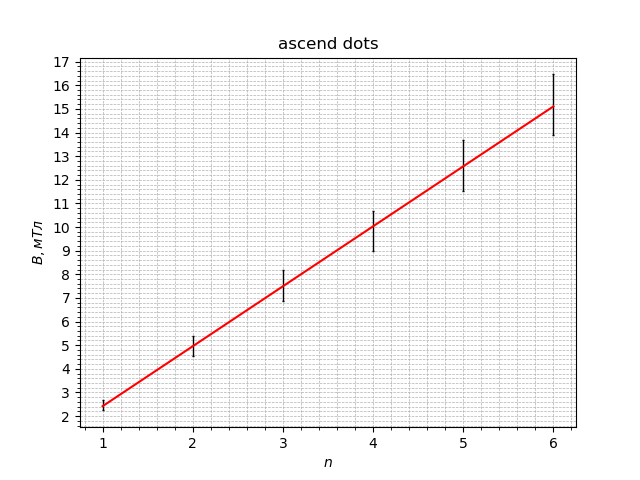
\includegraphics[width = 0.6\textwidth]{data/focus/graphs/ascend_dots.png}\\
    \textbf{График 4.} $B(n)$ в обратном направлении.
\end{center}

\begin{equation}
    k_{B/n} = (2.52 \pm 0.21) \; \frac{\text{мТл}}{\text{А}} \; (\varepsilon = 8 \%)
\end{equation}

\begin{equation}
    V = 0.97 \; \text{кВ}, \; \; \; l = 26.5 \; \text{см}
\end{equation}

Подставляя в формулу $(1)$ мы получаем, что
\begin{equation}
\dfrac{e}{m} = \left(1.72 \pm 0.15\right) \cdot 10^{11} \; \frac{\text{Кл}}{\text{кг}}
\end{equation}

Это значение очень близко к реальному $e/m = 1.76 \cdot 10^{11} \text{Кл}/\text{кг}$

\newpage

\section*{B. Метод магнетрона}
\subsection*{Цель работы:}
Исследование зависимости анодного тока от тока, протекающего через соленоид при различных напряжениях на аноде лампы и по результатам измерений рассчитать удельный заряд электрона $e/m$.
\subsection*{В работе используются:}
Электронная лампа с цилиндрическим анодом; соленоид; источники питания лампы и соленоида; вольтметр постоянного тока; миллиамперметр, амперметр.
\subsection*{Теоретическая справка}
Здесь удельный заряд электрона определяется по формуле
\begin{equation}
\dfrac{e}{m_e} = \dfrac{8V_a}{B_{\text{кр}}^2r_a^2},
\end{equation}
где $V_a$ - анодное напряжение, $B_{\text{кр}}$ - критическое поле, $r_a$ - радиус анода.
\subsection*{Описание установки.}
\begin{wrapfigure}{l}{0.3\textwidth}
  \begin{center}
    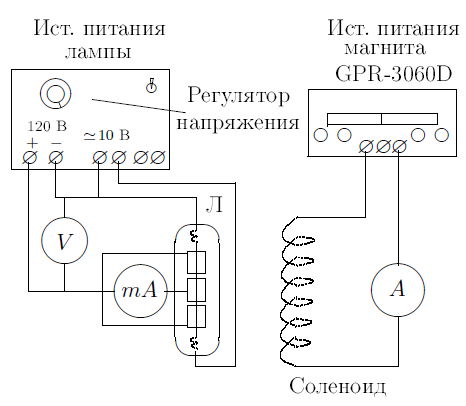
\includegraphics[width = 0.3\textwidth]{pictures/ustb.png}
  \end{center}
  \textbf{\caption{Схема установки.}}
\end{wrapfigure}
Два крайних цилиндра изолированы от среднего небольшими зазорами и используются для устранения краевых эффектов на торцах среднего цилиндра, ток с которого используется при измерениях. В качестве катода используется тонкая вольфрамовая проволока. Катод разогревается переменным током, отбираемым от стабилизированного источника питания.

С этого же источника на анод лампы подается напряжение, регулируемое с помощью потенциометра и измеряемое вольтметром.

Индукция магнитного поля в соленоиде рассчитывается по току $I_m$, протекающему через обмотку соленоида. Коэффициент пропорциональности между ними указан в установке.

Лампа закреплена в соленоиде. Магнитное поле в соленоиде создается постоянным током, сила которого регулируется ручками источника питания и измеряется амперметром.

\newpage
\;
\subsection*{Ход работы}

\end{document}
